\documentclass[../tesis.tex]{subfiles}
\begin{document}

% Ruta de imagenes para compilacion independiente o desde el archivo principal
\graphicspath{{../imagenes/}{imagenes/}}

\chapter{Evaluación de LLMs multimodales en la generación de informes mediante un LLM juez}
\label{cap:Capitulo4}

\section{Generación libre de informes radiológicos mediante MedGemma}
\label{sec:generacion_libre_medgemma}

Ante el modesto desempeño observado en los modelos multimodales al ser restringidos a tareas de clasificación cerrada mediante etiquetas rígidas (Capítulo 3), se propuso evaluar la capacidad de los modelos de visión y lenguaje (\textit{Vision-Language Models}, VLMs) para generar informes radiológicos completos en lenguaje natural. Bajo este esquema, los hallazgos clínicos son extraídos posteriormente a partir del texto generado para compararlos contra los informes de referencia (\textit{ground truth}). Dado que esta evaluación debe ejecutarse de forma masiva sobre una cohorte de $2\,818$ pacientes, se implementó un pipeline automatizado de evaluación semántica asistido por un LLM actuando como juez experto, seleccionando para dicha tarea el modelo \texttt{Qwen2.5-14B-Instruct}.

\subsection{Diseño del prompt para la generación restringida de informes radiológicos}
\label{subsec:prompt_informes}

A diferencia de la clasificación estructurada, la generación libre de texto en el dominio médico presenta un riesgo elevado de introducir redundancias, vaguedades o alucinaciones clínicas \citep{Artsi_et_al._2025} \citep{Doshi_et_al._2024}. Para mitigar estas desviaciones y acotar la salida al estilo sintético de un informe profesional, se diseñó un \textit{prompt} condicionado por directrices radiológicas estrictas.

Como se detalla en el \autoref{lst:prompt_informes}, la construcción de la instrucción inyecta dinámicamente los metadatos del paciente (sexo y proyecciones disponibles, e.g., PA, Lateral) e impone reglas operativas rigurosas:

\begin{itemize}
    \item \textbf{Penalización de Falsos Positivos:} Se establece que la inclusión de un falso positivo genera mayor perjuicio clínico que la omisión de un hallazgo dudoso, forzando al modelo a reportar exclusivamente anomalías confirmadas de forma inequívoca.
    \item \textbf{Control de Formato y Estilo:} Se limita la extensión a un máximo de cuatro oraciones cortas, prohibiendo frases genéricas o redundantes (e.g., \textit{"lungs are clear"}), viñetas, explicaciones etiológicas o recomendaciones terapéuticas.
    \item \textbf{Ejemplos de Referencia (\textit{Few-Shot Guidance}):} Se incorporan ejemplos explícitos del estilo sintáctico y la terminología esperada en el informe.
\end{itemize}

\subsection{Configuración de hiperparámetros e inferencia del modelo}
\label{subsec:inferencia_ollama}
Para el proceso de inferencia masiva se utilizó la API local de \textbf{Ollama}, evaluando las variantes \texttt{medgemma\_4b\_q6} y \texttt{medgemma:latest}. Con el fin de garantizar la reproductibilidad y consistencia técnica durante todo el conjunto de prueba, se fijaron parámetros de decodificación específicos (\autoref{lst:ollama_inference}):
\begin{itemize}
    \item \textbf{Temperatura ($\tau = 0{,}1$):} Se configuró un valor bajo para reducir el muestreo estocástico y favorecer una decodificación casi determinista, priorizando la precisión diagnóstica sobre la diversidad léxica.
    \item \textbf{Límite de Generación (\texttt{num\_predict = 120}):} Se acotó la ventana máxima a 120 tokens para asegurar el cumplimiento del límite de oraciones y prevenir bucles de repetición o texto accesorio.
\end{itemize}

\section{Evaluación semántica basada en LLM como juez (Qwen2.5-14B-Instruct)}
\label{sec:qwen_llm_juez}

Qwen es una familia de modelos de lenguaje de gran tamaño desarrollada por Alibaba Cloud. En particular, \texttt{Qwen2.5-14B-Instruct} es un modelo autorregresivo denso de 14 mil millones de parámetros que destaca por sus capacidades de razonamiento lógico, estructuración de salidas en formato JSON y seguimiento estricto de instrucciones complejas.

Debido al tamaño del modelo y a los requerimientos de memoria de video, la ejecución de Qwen2.5 no se realizó de forma local mediante Ollama, sino que se desplegó en el supercomputador \textbf{Clementina XXI} haciendo uso de bibliotecas nativas de aprendizaje profundo (\textit{PyTorch} y \textit{Hugging Face Transformers}).

\subsection{Criterios de evaluación cualitativa y construcción del prompt evaluador}
\label{subsec:prompt_juez}

Las métricas léxicas tradicionales de procesamiento de lenguaje natural (e.g., BLEU, ROUGE) resultan inadecuadas para evaluar informes radiológicos, ya que no capturan la equivalencia clínica ni penalizan adecuadamente las contradicciones diagnósticas (por ejemplo, alterar la frase \textit{"sin neumotórax"} por \textit{"neumotórax presente"} supone la modificación de una sola palabra pero representa un error clínico crítico) \citep{Artsi_et_al._2025}.

Para resolver esta limitación y alinear la evaluación con el rendimiento clínico real \citep{Doshi_et_al._2024}, se implementó una metodología de evaluación basada en un LLM actuando como juez experto (\textit{LLM-as-a-Judge}). Como se detalla en el \autoref{lst:prompt_juez}, el juez fue instruido mediante un \textit{prompt} estructurado para extraer los hallazgos clínicos significativos de cada informe generado y compararlos contra el informe original:

\begin{itemize}
    \item \textbf{Equivalencia Semántica:} Se instruye al modelo para tratar como equivalentes aquellas descripciones que expresen el mismo cuadro clínico, independientemente de la sintaxis empleada (e.g., \textit{"No active parenchymal processes"} $\equiv$ \textit{"Lungs are clear"}).
    \item \textbf{Filtrado de Hallazgos Normales y Descriptores Anatómicos:} Para evitar sobredimensionar la precisión, se definió una lista explícita de expresiones no patológicas y descriptores anatómicos normales (e.g., \textit{"preserved cardiothoracic ratio"}, \textit{"no pneumothorax"}) que son ignorados en el cómputo de métricas.
    \item \textbf{Regla de Contradicción y Manejo Vascular:} Se fijaron reglas lógicas para penalizar hallazgos contradictorios (donde un hallazgo omitido se asigna como FN y la afirmación opuesta inventada como FP) y se estandarizó la evaluación de alteraciones vasculares frecuentes como \textit{"aorta uncoiled"}.
    \item \textbf{Salida Estructurada JSON:} Se exigió una respuesta en formato JSON estricto sin texto razonado secundario (\texttt{/no\_think}), garantizando la automatización del parseo y la extracción cuantitativa de verdaderos positivos (TP), falsos positivos (FP) y falsos negativos (FN).
\end{itemize}



\subsection{Infraestructura computacional y despliegue en el supercomputador Clementina XXI}
\label{subsec:clementina_xxi}

El procesamiento masivo del conjunto de datos y la ejecución del modelo evaluador \texttt{Qwen2.5-14B-Instruct} se llevaron a cabo en el cluster de supercomputación \textbf{Clementina XXI}. Dado que el entorno dispone de aceleradores gráficos de arquitectura Intel Data Center GPU Max (\texttt{intel\_xt1550}), el pipeline de inferencia se adaptó utilizando la pila de controladores Intel oneAPI y el soporte nativo para el backend de ejecución \texttt{xpu} en PyTorch.

En el \autoref{lst:slurm_script} se muestra el script de trabajo para el gestor de recursos SLURM, donde se destacan los siguientes parámetros de configuración:

\begin{itemize}
    \item \textbf{Asignación de Recursos Hardware:} Se solicitó un nodo de cómputo configurado con 16 núcleos de CPU, 128 GB de memoria RAM y una GPU Intel Data Center (\texttt{gres=gpu:intel\_xt1550:1}).
    \item \textbf{Entorno de Ejecución Intel oneAPI:} Se cargaron las librerías dinámicas de tiempo de ejecución mediante la inclusión de \texttt{setvars.sh} (versión 2025.3) y la configuración explícita de variables de entorno para la pila SYCL y Level Zero (\texttt{ONEAPI\_DEVICE\_SELECTOR=level\_zero:gpu}).
    \item \textbf{Inferencia con Precisión Mixta:} La carga del modelo en memoria de video se realizó empleando precisión \texttt{torch.bfloat16} mapeada directamente sobre el dispositivo \texttt{torch.device("xpu")}, optimizando el rendimiento y reduciendo la huella de memoria en el acelerador.
\end{itemize}



\section{Evaluación del desempeño del LLM juez y resultados del benchmark}
\label{sec:eval_juez_benchmark}

La función del modelo \texttt{Qwen2.5-14B-Instruct} consistió en comparar los informes generados por los VLMs contra los informes originales, extrayendo las etiquetas de verdaderos positivos (TP), falsos positivos (FP) y falsos negativos (FN). Durante la ejecución sobre los $2\,818$ pacientes, el evaluador automático registró únicamente dos fallos de parseo, los cuales fueron resueltos manualmente.

Para estimar la fiabilidad del juez automático, se realizó una auditoría cualitativa manual sobre una muestra representativa de 100 pacientes. Dado que no se contó con la participación directa de un especialista radiólogo para esta verificación, el proceso se apoyó en el modelo fundacional \textbf{Gemini} (Google) como herramienta de soporte técnico para el análisis semántico acelerado, siendo cada una de las clasificaciones, discrepancias y decisiones finales auditadas y consolidadas de forma manual por el autor.

La auditoría reveló que \texttt{Qwen2.5-14B-Instruct} presentó un desempeño totalmente correcto en aproximadamente el $80\%$ de las evaluaciones. La categorización detallada de los errores ($20\%$ restante) se distribuyó de la siguiente manera:
\begin{itemize}
    \item \textbf{Errores Leves ($8\%$):} Diferencias de redacción o interpretación sintáctica menor que no modifican la evaluación clínica ni alteran significativamente las métricas.
    \item \textbf{Errores Moderados ($8\%$):} Clasificación incorrecta de TP, FN o FP asociada a hallazgos secundarios o equivalencias semánticas discutibles.
    \item \textbf{Errores Graves ($4\%$):} Omisión o aceptación incorrecta de hallazgos clínicamente relevantes que alteran directamente el cómputo global.
\end{itemize}

Un hallazgo crucial de esta auditoría fue que los errores del juez automático no se comportaron como un ruido estocástico o simétrico, sino que evidenciaron un \textbf{sesgo sistemático por sobre-rigidez sintáctica}. Específicamente, Qwen tendió a sobre-generar falsos negativos (FN) al penalizar formulaciones sintácticas válidas de \textit{MedGemma} por no coincidir literalmente con la redacción del informe de referencia (por ejemplo, no equiparar \textit{``enlarged cardiac silhouette''} con \textit{``cardiomegaly''}), e infló los falsos positivos (FP) al clasificar descriptores anatómicos como hallazgos alucinados.

Dado que los falsos negativos y falsos positivos se ubican en el denominador de las métricas de \textit{Recall} ($\frac{\text{TP}}{\text{TP} + \text{FN}}$), \textit{Precision} ($\frac{\text{TP}}{\text{TP} + \text{FP}}$) y \textit{Exact Match}, la hiper-rigidez del juez subestimó sistemáticamente el desempeño real de los modelos en bruto.

Los márgenes de desvío estimados sobre la muestra auditada registraron:
\begin{itemize}
    \item Para \texttt{medgemma\_4b\_q6}: desvío de $10{,}04\%$ en TP, $10{,}02\%$ en FP y $27{,}06\%$ en FN.
    \item Para \texttt{medgemma\_latest}: desvío de $6{,}92\%$ en TP, $4{,}80\%$ en FP y $24{,}20\%$ en FN.
\end{itemize}

Al compensar el sesgo direccional de Qwen mediante la restitución de las equivalencias semánticas penalizadas por error, se obtuvieron los resultados proyectados para el pipeline en generación libre. El resultado principal de este benchmark se establece a partir de las métricas brutas (directas) reportadas por el LLM juez, las cuales sitúan a MedGemma 4B Q6 en un Micro F1 de $0{,}69$ y un Exact Match de $0{,}43$ (y $0{,}68$ / $0{,}41$ para MedGemma Latest), tal como se detalla en la \autoref{tab:benchmark_corregido}. 

Complementariamente, para cuantificar el impacto de las discrepancias del juez, la auditoría sobre los 100 casos se enmarca formalmente como un \textbf{análisis exploratorio de sesgo y discrepancia del juez}. A partir de los desvíos detectados por sobre-rigidez sintáctica, se calculó una estimación proyectada que representa una \textbf{cota teórica superior sujeta a validación ciega por especialistas radiólogos}. La comparativa entre las métricas brutas principales y dicha proyección ajustada se presenta en la \autoref{tab:benchmark_corregido}.

\begin{table}[htbp]
\centering
\small
\begin{tabular}{llcc}
\hline
\textbf{Modelo} & \textbf{Métrica} & \textbf{\begin{tabular}[c]{@{}c@{}}Evaluación Bruta\\ (Resultado Principal)\end{tabular}} & \textbf{\begin{tabular}[c]{@{}c@{}}Proyección Ajustada\\ (Cota Superior Teórica)*\end{tabular}} \\
\hline
\textbf{MedGemma 4B Q6}   & Precisión   & 0.68 & 0.72 \\
(\texttt{medgemma\_4b\_q6}) & Recall      & 0.70 & 0.78 \\
                         & Micro F1    & \textbf{0.69} & 0.75 \\
                         & Exact Match & \textbf{0.43} & 0.59 \\
\hline
\textbf{MedGemma Latest}  & Precisión   & 0.69 & 0.72 \\
(\texttt{medgemma\_latest}) & Recall      & 0.66 & 0.73 \\
                         & Micro F1    & \textbf{0.68} & 0.72 \\
                         & Exact Match & \textbf{0.41} & 0.59 \\
\hline
\end{tabular}
\caption{Resultados del benchmark radiológico en generación libre: comparativa entre las métricas brutas principales de Qwen2.5-14B y la cota superior proyectada mediante análisis exploratorio de sesgo ($N = 2\,818$). *\small{La proyección ajustada constituye una cota teórica superior sujeta a validación ciega por radiólogos.}}
\label{tab:benchmark_corregido}
\end{table}

Cabe destacar que no se realizó un análisis estratificado por patología individual debido a que el evaluador automático produce descripciones en lenguaje natural sin una ontología cerrada, lo que dificulta agrupar homogéneamente términos equivalentes (e.g., \textit{``cardiomegaly''}, \textit{``increase in transverse cardiac diameter''} y \textit{``borderline enlarged heart''}). Por tanto, la evaluación se reporta mediante métricas multietiqueta globales.

\section{Discusión y conclusiones del capítulo}
\label{sec:discusion_ch4}

Como se puede observar en la \autoref{fig:comparacion_generacion}, los resultados sugieren una divergencia en el comportamiento de los modelos bajo distintos esquemas de salida. No obstante, dado que en esta comparación cambian simultáneamente la tarea (clasificación estructurada frente a redacción de texto), la naturaleza de la referencia y el mecanismo evaluador (métricas de coincidencia estricta frente a un LLM juez), estas diferencias deben interpretarse estrictamente como una observación exploratoria sobre la respuesta de los modelos ante formatos de salida alternativos, sin afirmar una superioridad metodológica absoluta de un paradigma sobre otro.
\begin{figure}[htbp]
\centering
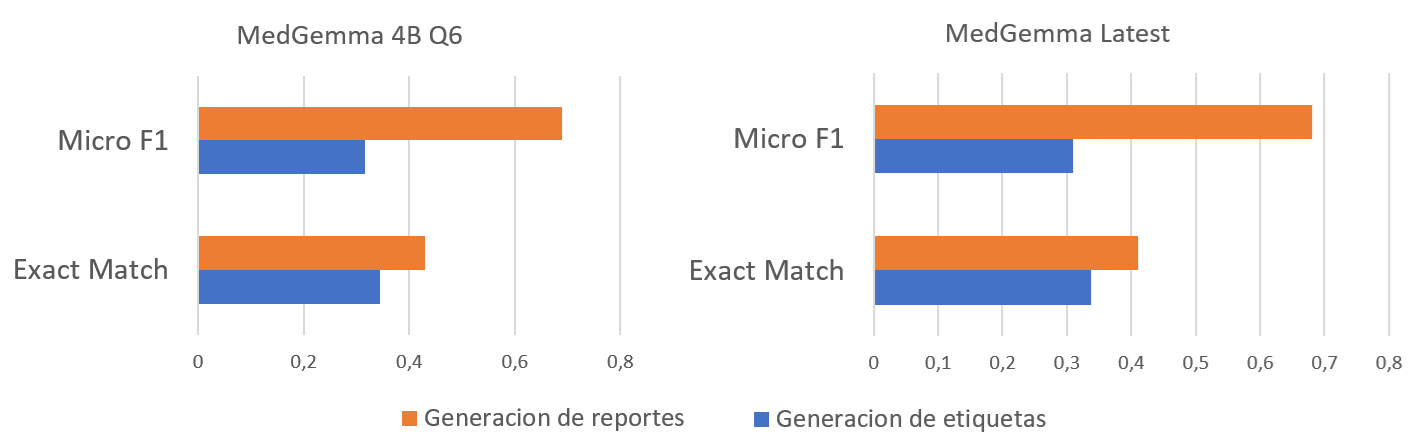
\includegraphics[width=1\textwidth]{Tesis/comparacio_generacion.png}
\caption{Comparativa del rendimiento en términos de Exact Match y Micro F1 entre la generación estructurada de etiquetas (salidas estrictas) y la generación libre de reportes para ambos modelos MedGemma tomando los valores reportados por el juez (Qwen).}
\label{fig:comparacion_generacion}
\end{figure}

Alcanzar un desempeño principal en bruto de $0{,}43$ en Exact Match y $0{,}69$ en Micro F1 utilizando un modelo liviano de 4 mil millones de parámetros constituye el hallazgo central del benchmark, especialmente considerando la disponibilidad de arquitecturas médicas de mayor escala. Por ejemplo, modelos especializados desarrollados recientemente, como MAIRA-2 \citep{bannur2024maira2groundedradiologyreport} y su evolución MAIRA-X \citep{sharma2025closingperformancegapai}, han alcanzado valores de hasta 0,80 en generación de informes y 0,90 en localización visual (Grounding Recall). Si bien el análisis exploratorio de sesgo proyecta una cota teórica superior de hasta $59\%$ en Exact Match bajo corrección del juez, dicha estimación debe interpretarse con estricta cautela como un límite superior teórico pendiente de validación ciega por especialistas radiólogos.

A partir de los resultados obtenidos, la incorporación de un MLLM generador representa una alternativa viable dentro de un pipeline radiológico modular. En este esquema, el modelo de lenguaje puede integrarse con módulos especializados de visión que detecten patologías específicas y le proporcionen información estructurada, la cual es combinada con el historial clínico, los síntomas y los metadatos del paciente para redactar el informe final. 

Sin embargo, confiar la redacción autónoma de un informe diagnóstico exclusivamente a un MLLM a partir de la radiografía resulta una pretensión prematura en el contexto actual. Ninguna agencia regulatoria de alta exigencia (como la FDA en EE. UU. o la EMA en Europa) ha aprobado hasta el momento el uso autónomo e independiente de modelos de lenguaje multimodales para la emisión de diagnósticos primarios sin supervisión profesional \citep{Artsi2025Large}.


\end{document}